\section{Распространение фотона в замагниченной плазме}

Распространение фотона в активной среде удобнее всего описывать в терминах собственных функций (задающих возможные его поляризационные состояния) и собственных значений (определяющих дисперсионные свойства) поляризационного оператора фотона ${\cal P}_{\alpha\beta}$, явный вид которого может быть получен из результатов работ~\cite{Shabad:1988,Tsai:1974,Batalin:1971,Skobelev:1975}. Для дальнейшего анализа получим его разложение по базису, построенному на 4-векторе импульса фотона, $q_\mu$, и обезразмеренном тензоре электромагнитного поля, $\varphi_{\alpha\beta}=F_{\alpha\beta}/B$. В системе отсчета, в которой имеется только магнитное поле, индукция которого направлена вдоль оси $z$, тензор $\varphi_{\alpha\beta}$ и дуальный к нему $\tilde{\varphi}_{\alpha\beta}=\frac{1}{2}\varepsilon_{\alpha\beta\mu\nu} \varphi^{\mu\nu}$, принимают следующий вид:
%
\beq
\varphi_{\alpha\beta} = \begin{pmatrix} 0 & 0 & 0 & 0 \\ 0 & 0 & -1 & 0 \\ 0 & 1 & 0 & 0 \\ 0 & 0 & 0 & 0 \end{pmatrix} \, , \quad
\tilde{\varphi}_{\alpha\beta} = \begin{pmatrix} 0 & 0 & 0 & 1 \\ 0 & 0 & 0 & 0 \\ 0 & 0 & 0 & 0 \\ -1 & 0 & 0 & 0 \end{pmatrix} \, .
\eeq
%

Составленные из них конструкции: $\Lambda_{\alpha \beta} = (\varphi\varphi)_{\alpha\beta} = \mbox{diag}(0, 1, 1, 0)$ и $\widetilde \Lambda_{\alpha \beta} = (\widetilde\varphi\widetilde\varphi)_{\alpha\beta} = \mbox{diag}(1, 0, 0, -1)$ позволяют разбить четырехмерное пространство-время на подпространства Евклида \{1, 2\} и Минковского \{0, 3\}, обозначенные символами $\bot$ и $\parallel$, соответственно. Тогда для произвольных векторов имеем:
\beq
p_{\mprp}^\mu = (0, p_1, p_2, 0), \quad p_{\mprl}^\mu = (p_0, 0, 0, p_3),
\\
\nonumber
(pq)_{\mprp} = (p \Lambda q) =  p_1 q_1 + p_2 q_2, 
\\
\nonumber (pq)_{\mprl}= (p \widetilde \Lambda q) = p_0 q_0 - p_3 q_3.
\eeq

В качестве векторов, на которых мы построим базис для разложения поляризационного оператора фотона, выберем собственные векторы поляризационного оператора в постоянном однородном магнитном поле~\cite{Batalin:1971}:
\beq
\label{eq:basis}
b_{\mu}^{(1)} = (\varphi q)_\mu, \qquad
 b_{\mu}^{(2)} = (\tilde \varphi q)_\mu, 
\\
\nonumber
b_{\mu}^{(3)} = q^2 \, (\Lambda q)_\mu - q_\mu \, q^2_{\mbox{\tiny $\bot$}}, 
\qquad b_{\mu}^{(4)} = q_\mu, 
\eeq 

Этот базис не является нормированным, модули векторов имеют следующие значения:
\beq
\label{eq:basis_norm}
(b^{(1)} b^{*(1)}) = -q^2_{\mprp}, \quad
(b^{(2)} b^{*(2)}) = -q^2_{\mprl}, 
\\
\nonumber
 (b^{(3)} b^{*(3)}) = -q^2 q^2_{\mprl} 
q^2_{\mprp}, \quad (b^{(4)} b^{*(4)}) = q^2. 
\eeq

В замагниченной плазме ${\cal P}_{\alpha \beta}$ уже не будет диагональным в базисе из векторов~(\ref{eq:basis}), поэтому его удобно разложить  по собственным векторам $r_{\alpha}^{(\lambda)}$ в замагниченной плазме с соответствующими собственными 
значениями ${\cal P}^{(\lambda)}$~\cite{Rojas1979r,Rojas1982,Shabad:1988,MRCh:2014}:
%
\beq
\label{eq:Pab10}
{\cal P}_{\alpha \beta} = \sum_{\lambda = 1}^{3} 
{\cal P}^{(\lambda)} \, \frac{r_{\alpha}^{(\lambda)} 
	(r_{\beta}^{(\lambda)})^{*}}{(r^{(\lambda)})^2} \, , \quad 
r_{\beta}^{(\lambda)} = \sum\limits_{i = 1}^{3} A_i^{(\lambda)} \, b_{\beta}^{(i)} \, , 
\eeq
\noindent где  $A_i^{(\lambda)}$ -- некоторые комплексные коэффициенты.

Нахождение вида разложения~\ref{eq:Pab10} для случая замагниченной плазмы с произвольными характеристиками сопряжено со значительными вычислительными сложностями, поэтому эта задача решалась для случаев, когда один из параметров доминирует над другими. Так, в случае магнитодоминирующей среды (см. Введение), используя результаты  работ~\cite{Rojas1979, Rojas1982 ,Rojas1979r, Shabad:1988, MRCh:2014}, в кинематической области вдали от циклотронных резонансов, $q^2_{\mprl} \ll (m_e+\sqrt{m_e^2+2 \beta})^2$, можно получить следующее разложение:
%
\beq
\nonumber
&&{\cal P}_{\alpha \beta}  
 \simeq 
 - \frac{2\alpha}{\pi} \; \beta \, {\cal D} \, 
\frac{(\tilde \varphi q)_\alpha (\tilde \varphi q)_\beta}{q^2_{\mprl}} 
+ 
\frac{\alpha}{3\pi}\; (\varphi q)_\alpha (\varphi q)_\beta +
\frac{\ii \alpha}{\pi} \, \Delta N \, \big [
\varphi_{\alpha \beta} \, (qu) + (q\varphi)_{\alpha} u_{\beta} - 
\\
\label{eq:Pab1}
&&-
(q\varphi)_{\beta} u_{\alpha} \big ]  +
 \frac{\alpha}{3\pi} \, {\cal V} \, \left (q^2 \, g_{\alpha \beta} - 
q_{\alpha} \, q_{\beta} \right )  + 
O \left (\frac{1}{\beta} \right) \, , 
\eeq  
\noindent где 
%
\beq
\label{eq:PabD}
{\cal D} = - {\cal J} (q_{\mprl})  - 
H \left (\frac{q^2_{\mprl}}{4m^2} \right)  \, , 
\eeq
%
\beq
\label{eq:PabJ}
{\cal J} (q_{\mprl}) = 2q^2_{\mprl} \, m^2 \, \int\limits_{-\infty}^{\infty}  \frac{\dd p_z}{E} \, 
\frac{f_{-}(p) + f_{+}(p)}{q_{\mprl}^4 - 4(pq)^2_{\mprl}} \, , 
\eeq
%
\beq
\label{eq:fermidist}
&&f_{\pm}(p) = \frac{1}{1+\exp{[((pu)_{\mprl} \pm \mu)/T]}} \, , 
\\ [3mm]
\nonumber
&&
\quad (pu)_{\mprl} = E u_0 - p_z u_z \, , \quad E=\sqrt{p_z^2+m_e^2} \, .
\eeq
\noindent Здесь $u^{\mu}$ -- 4-вектор скорости плазмы, верхний знак соответствует электронной компоненте плазмы, нижний -- позитронной.

%
\beq
\label{eq:H0}
\nonumber
&&H(z)=\frac{1}{\sqrt{z(1 - z)}} \, \arctg \sqrt{\frac{z}{1 - z}} - 1, \quad 0 \leqslant z \leqslant 1 \, ,
\label{eq:H1}
\eeq
%
\beq
\nonumber
\Delta N &=& \int\limits_{-\infty}^{\infty}  \frac{\dd p_z}{E} 
\, (pu)_{\mprl} \, \left [f_{-}(p) - f_{+}(p) \right] = 
\frac{(2 \pi)^2}{\beta} \, (n_{e} - n_{e^+}) \, ,
\label{eq:PabA}  
\eeq
%
\beq
\label{eq:Lambda}
{\cal V} = \ln{(B/B_e)} - 1.792 + 
\frac{3}{2} \, \int\limits_0^1 \dd x \, (1-x^2) \, 
\ln{\left [1- \frac{q^2}{4m_e^2} \, (1-x^2) \right ]} \, .
\eeq

В данном обзоре рассматривается система покоя плазмы, так, что\\ $(pu)_{\mprl} = E$. При этом в разложении собственных векторов $r^{(\lambda)}_{\alpha}$ по обратным степеням поля для получения самосогласованных результатов  оказывается необходимым  учесть следующий порядок малости по $1/\beta$. С учетом этих замечаний получим:  
%
\beq
\label{eq:r13}
&&r^{(1,3)}_{\alpha} = \left [\mp \sqrt{q^4_{\mprp} + 
	(6 \Delta N \, \omega)^2\, \frac{q^2}{q_{\mprl}^2}}  - q^2_{\mprp} \right ]\, 
b^{(1)}_{\alpha} - \ii \, \frac{6 \Delta N \, \omega}{q_{\mprl}^2} \,  b^{(3)}_{\alpha} +
\\
\nonumber 
&&+ \ii \,\frac{\Delta N \, k_z \, q^2_{\mprp}}{2\beta \, {\cal D} \, q^2_{\mprl}}\, 
\left [\pm \sqrt{q^4_{\mprp} + 
	(6 \Delta N \, \omega)^2\, \frac{q^2}{q_{\mprl}^2}} + q^2_{\mprp} \right ]\; b^{(2)}_{\alpha} + 
O \left (\frac{1}{\beta^2} \right) \, ,
\eeq
%
\beq
\label{eq:r2}
r^{(2)}_{\alpha} =  b^{(2)}_{\alpha} - 
\ii \, \frac{\Delta N  \, k_z }{2\beta \, {\cal D}} \, b^{(1)}_{\alpha} + 
O \left (\frac{1}{\beta^2} \right)  \, .
\eeq


Коэффициенты $A_i^{(\lambda)}$ в разложении~(\ref{eq:Pab10}) с 
точностью до членов $O(1/\beta^2)$ имеют вид:
%
\beq
\label{eq:Ailambda}
&&A_1^{(1,3)} =  \mp \sqrt{q^4_{\mprp} + (6 \Delta N \, \omega)^2\, \frac{q^2}{q_{\mprl}^2}}  - q^2_{\mprp} \, ,
\\[3mm]
\nonumber
&&A_2^{(1,3)}  = \ii \,\frac{\Delta N \, k_z \, q^2_{\mprp}}{2\beta \, {\cal D} \, q^2_{\mprl}}\, 
\left [\pm \sqrt{q^4_{\mprp} + 
	(6 \Delta N \, \omega)^2\, \frac{q^2}{q_{\mprl}^2}} + q^2_{\mprp} \right ] \, ,
\\[3mm]
\nonumber
&&A_3^{(1,3)} = - \ii \, \frac{6 \Delta N \, \omega}{q_{\mprl}^2} \, , \quad  
A_1^{(2)} = - \ii \, \frac{\Delta N  \, k_z }{2\beta \, {\cal D}} \, ,
\\[3mm]
\nonumber
&&A_2^{(2)} = 1 \, , \quad  A_3^{(2)} = 0 \, .
\eeq

Соответствующие собственные значения в приближениях $O(1/\beta^2)$ для ${\cal P}^{(1,3)}$ и
$O(1/\beta)$ для ${\cal P}^{(2)}$ запишутся следующим образом:
\beq
\label{eq:kappa13}
{\cal P}^{(1,3)} = \frac{\alpha}{3\pi} \, q^2 \, {\cal V} + 
\frac{\alpha}{6\pi} \, \left [ 
 \mp \sqrt{q^4_{\mprp} + 
(6 \Delta N \, \omega)^2\, \frac{q^2}{q_{\mprl}^2}}  - q^2_{\mprp} \right ]  
+ O \left (\frac{1}{\beta} \right)  \, ,
\eeq
%
\beq
\label{eq:kappa2}
{\cal P}^{(2)} = \frac{\alpha}{3\pi} \, q^2 \, {\cal V} + \frac{2 \alpha}{\pi} \, \beta \, {\cal D}  + 
 O \left (\frac{1}{\beta} \right) \, .
\eeq

Как видно из полученного результата, даже в приближении сильно замагниченной плазмы 
определение дисперсионных свойств фотонов для всех трех поляризаций  
представляет собой достаточно сложную задачу.  Однако в предельном случае зарядово-симметричной
плазмы формулы~(\ref{eq:Ailambda}) -- (\ref{eq:kappa2}) значительно упрощаются. 

А именно, в случае зарядово-симметричной плазмы, $\Delta N = 0$, а также в случае холодной, почти вырожденной, умеренно релятивистской плазмы при выполнении условия $\Delta N /(2m_e) \simeq v_F \ll 1$, где $v_F$ соответствует скорости частицы, находящейся на уровне Ферми, коэффициенты~(\ref{eq:Ailambda}) примут вид: $A_1^{(1)} = -2 q^2_{\mprp}$, $A_2^{(2)} = 1$ (остальные коэффициенты равны нулю). Тогда собственные векторы~(\ref{eq:r13}) -- (\ref{eq:r2}) и 
собственные значения~(\ref{eq:kappa13}) -- (\ref{eq:kappa2}) можно представить в виде:
%
\beq
\label{eq:r132}
r^{(1)}_{\alpha} =  -2 q^2_{\mprp} \, b^{(1)}_{\alpha}  + O \left (\frac{1}{\beta^2} \right) \, ,
 \quad 
%\eeq
%
%\beq
%\label{eq:r20}
r^{(2)}_{\alpha} =  b^{(2)}_{\alpha}  + O \left (\frac{1}{\beta^2} \right)  \, .
\eeq
%
\beq
\label{eq:kappa10}
&&{\cal P}^{(1)} = \frac{\alpha}{3\pi} \, q^2 \, {\cal V} - \frac{\alpha}{3\pi} \, 
q^2_{\mprp} + O \left (\frac{1}{\beta} \right)  \, ,
\\[3mm]
\label{eq:kappa30}
&&{\cal P}^{(3)} = \frac{\alpha}{3\pi} \, q^2 \, {\cal V} + O \left (\frac{1}{\beta} \right)  \, ,
\eeq
%
\noindent а собственное значение  ${\cal P}^{(2)}$ определяется формулой~(\ref{eq:kappa2}). Вектор $r^{(3)}_{\alpha} \sim  O \left (1/\beta^2\right)$ и, следовательно, не может соответствовать фотону с определенным поляризационным состоянием.

\begin{figure}[t!]
	\centerline{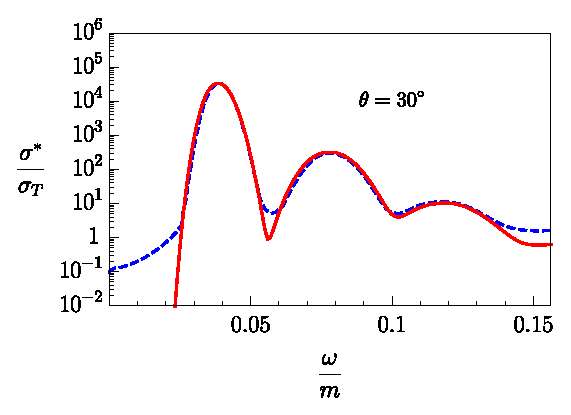
\includegraphics[width = 15cm]{fig2_1.eps}}
	\vspace*{-2mm} \caption{Законы дисперсии фотона моды 2 в сильном магнитном поле  $B/B_e = 200$  
		и нейтральной плазме ($\mu=0$) для различных значений температуры:  $T = 1$ МэВ 
		(верхняя кривая), $T = 0.5$ МэВ (средняя кривая), $T = 0.25$ МэВ (нижняя кривая). 
		Дисперсия фотона без плазмы обозначена штриховой линией.
		Диагональная штриховая линия соответствует вакуумному закону дисперсии, $q^2 = 0$. Угол
		между импульсом фотона  и направлением  магнитного поля равен 
		$\pi/2$. } 
	\label{fig:disT}
\end{figure}

Следует отметить, что полученные собственные векторы~(\ref{eq:r132}) не являются единичными, и для описания поляризационных состояний фотона удобнее использовать нормированные векторы:
%
\beq
\label{eq:epsilon}
%&&
\varepsilon_\alpha^{(1)}(q) = \frac{r^{(1)}_{\alpha}}{\sqrt{|(r^{(1)} r^{*(1)})|}} = 
\frac{(q \varphi)_\alpha}{\sqrt{q_{\mprp}^2}} \, , \quad
%\\
%\nonumber
%&&
\varepsilon_\alpha^{(2)}(q) = \frac{r^{(2)}_{\alpha}}{\sqrt{|(r^{(2)} r^{*(2)})|}} = 
\frac{(q \tilde \varphi)_\alpha}{\sqrt{q_{\mprl}^2}}.
\eeq
\noindent Здесь символы 1 и 2 соответствуют  $\|$ и $\perp$ --  поляризациям в чистом магнитном поле~\cite{Adler:1971}, $X$ - и $O$ -  модам работы~\cite{Mushtukov:2016}, и $E$ - и $O$ -  модам в замагниченной плазме~\cite{Thompson:1996}. Волновые функции фотона $A^{(\lambda)}_\mu(X)$ можно представить в виде плосковолновых решений:
%
\begin{eqnarray}
	\label{eq:j_k}
	A^{(\lambda)}_\mu (X) = \frac{e^{-\ii(qX)}}{\sqrt{2q_0 V}} \, \varepsilon^{(\lambda)}_\mu(q) \, ,
\end{eqnarray}
\noindent где  $V = L_x L_y L_z$ -- нормировочный объем и $\lambda = 1, 2$ -- мода фотона.

Нетрудно увидеть, что полученные таким образом собственные векторы и собственные значения поляризационного 
оператора в плазме с точностью до членов порядка  $O(1/\beta^2)$ and $O(\alpha^2)$ совпадают с соответствующими величинами в  замагниченном вакууме~\footnote{Под термином <<замагниченный вакуум>>  понимается магнитное поле без плазмы.}. Такой вывод находится в согласии с результатами работы~\cite{Shabad:1988} и, для предельного случая $\omega \ll m_e$ и после необходимых преобразований: выбора продольной составляющей $\varepsilon^{(2)}_\alpha$ и перехода в систему координат, в которой вектор импульса фотона направлен вдоль оси $z$, работы~\cite{Potekhin:2004}.

Закон дисперсии фотона моды 1 в приближении $O(1/\beta^2)$ практически не отличается от вакуумного, $q^2 \simeq 0$. Действительно, из закона дисперсии для этой моды:
%
\beq
q^2 - {\cal P}^{(1)} = 0 \, 
\label{disper1}
\eeq
\noindent и формулы~(\ref{eq:kappa10}) следует, что
%
\beq
q_{\mprl}^2 = \left (1- \frac{\alpha}{3\pi} \frac{1}{1-\frac{\alpha}{3\pi} \cal V} \right) \, q_{\mprp}^2  
\simeq q_{\mprp}^2 \left (1- \frac{\alpha}{3\pi} \right)\, , 
\label{disper12}
\eeq
\noindent так что $q^2 \simeq 0$, оставаясь при этом отрицательным. Кроме того, из формулы~(\ref{eq:kappa10}) следует, что в кинематической области $q^2_{\mprl} \ll (m_e+\sqrt{m_e^2+2 \beta})^2$ собственное значение поляризационного оператора моды 1 не имеет мнимой части~\footnote{Строго говоря, мнимая часть является сильно подавленной по сравнению с реальной частью, так что такой фотон будет квазистабильным.}

\begin{figure}[t]
	\centerline{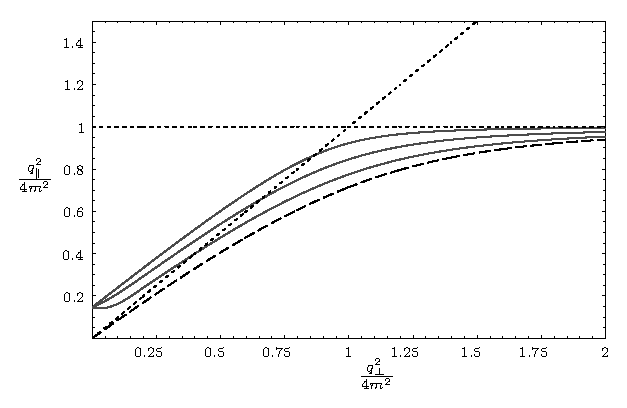
\includegraphics[width=15cm]{fig2_2.eps}} \vspace*{-2mm}
	\caption{Законы дисперсии фотона моды 2 в сильном магнитном поле  $B/B_e = 200$  
		и нейтральной плазме $(T = 1 \mbox{МэВ})$ для различных значений
		угла  между импульсом фотона  и направлением  магнитного поля
		$\theta = \pi/2$ (верхняя кривая), $\theta = \pi/6$  (средняя кривая), $\theta = \pi/12$
		(нижняя кривая).
		Дисперсия фотона без плазмы обозначена штриховой линией.
		Диагональная штриховая линия соответствует вакуумному закону дисперсии, $q^2 = 0$.
	}
	\label{fig:disTheta}
\end{figure}

С другой стороны, дисперсионные свойства фотона моды 2  претерпевают существенные изменения даже по сравнению с замагниченным вакуумом и, следовательно, будут оказывать дополнительное влияние на кинематику процессов с участием фотонов этой моды. На рис.~\ref{fig:disT} и~\ref{fig:disTheta} представлены законы дисперсии фотона моды 2 в замагниченной зарядово-симметричной ($\mu=0$) плазме, для различных значений температур, углов и импульса фотона, полученные как решения уравнения
%
\beq
q^2 - {\cal P}^{(2)} = 0 \, .
\label{disper}
\eeq
\noindent Как нетрудно видеть, в противоположность чистому 
магнитному полю, в плазме существует область с  $q^2 > 0$ ниже  первого  
циклотронного резонанса, определяемого условием $q^2_{\mprl} = 4 m_e^2$. 

Этот факт связан  с появлением плазменной частоты в представлении реальных электронов и позитронов среды, 
которая может быть определена из уравнения
%
\begin{equation}
\omega_{p}^2 - {\cal P}^{(2)} (\omega_{p}, {\mathbf k} \to 0 ) = 0.
\label{eq:omegapl}
\end{equation}
%
Для случая сильно замагниченной зарядово-симметричной нерелятивистской плазмы можно получить приближенное решение этого уравнения. В результате мы получим классическое выражение $\omega_{pl}^2 \simeq 2(4\pi \alpha n_{e})/m_e$ (множитель 2 возникает из-за равенства концентраций электронов и позитронов), где
%
\begin{eqnarray}
n_{e} \simeq \beta \sqrt{\frac{m_e T}{(2\pi)^3}}\,e^{-m_e/T}.
\label{eq:ne}
\end{eqnarray}
\noindent Таким образом, $\omega_{pl}$ для зарядово-симметричной плазмы экспоненциально подавлено. С другой стороны, для зарядово-несимметричной плазмы подавление отсутствует и $\omega_{pl}^2 \simeq (2\alpha \beta/\pi)v_F$.

Тем не менее, даже для зарядово-симметричной плазмы при температуре $T=50$ КэВ и индукции магнитного поля $B=200 B_e$ мы получаем такую оценку для плазменной частоты: $\omega_{pl} \simeq 3$ КэВ, что уже может повлиять на кинематику различных процессов с участием фотона. Например, наличие плазменной частоты приводит к возникновению порога для каналов рассеяния фотона моды 2 на электронах и позитронах плазмы, $\gamma_2 e \to \gamma_1 e$, $\gamma_2 e \to \gamma_2 e$, который отсутствует в чистом магнитном поле. А для одной из основных реакций, в которых рождаются поляризованные фотоны, -- процесса расщепления фотона на два фотона, $\gamma \to \gamma \gamma$, оно приводит к возникновению новых правил отбора по поляризациям: в области ниже порога рождения $e^+e^-$-пар, $q^2_{\mprl} = 4 m^2$, и в области, где $q^2 > 0$, каналы, в которых рождаются фотоны моды 2, $\gamma_2 \to \gamma_2 \gamma_2$,
$\gamma_1 \to \gamma_2 \gamma_2$ и $\gamma_1 \to \gamma_1 \gamma_2$, кинематически закрыты и становится открытым новый канал $\gamma_2 \to \gamma_1 \gamma_1$, запрещенный в магнитном поле в отсутствие плазмы.

Пропагатор фотона определяется решением следующего волнового уравнения:
\begin{eqnarray}\label{eq:WaveEq}
	\nonumber
	&& 
	(g_{\alpha \rho} \, \partial_{\mu}^2  -
	\partial_{\alpha}\partial_{\rho}) \, G^{\rho}_{\phantom{x}\beta}(x) + 
	\int d^4 x'\, {\cal P}^{(\lambda)}_{\alpha\rho} (x - x') \, 
	G^{\rho}_{\phantom{x}\beta}(x)
	\nonumber= g_{\alpha\beta}\delta^4(x),
	\label{eq:2}
\end{eqnarray}
%                                                                                         \frac{(\varphi q)_\mu}{\sqrt{q^2_\perp}}
где $\delta^4(x)=\delta(t)\delta(x)\delta(y)\delta(z)$. 

В координатном пространстве пропагатор фотона можно представить следующим 
образом:
\begin{equation}\label{eq:InvGcFourier}
	G_{\mu\nu}(x)=\int \frac{\dd^4q}{(2\pi)^4}G_{\mu\nu}(q) e^{-\ii qx}\, ,
\end{equation}
где
\begin{equation}\label{eq:GcFourier}
	G_{\mu\nu}(q)=\sum_{\lambda=1}^{3}\frac{b_\mu^{(\lambda)}b^{(\lambda)}_\nu}{(b^{(\lambda)})^2}\cdot
	 \frac{1}{q^2-{\cal P}^{(\lambda)}(q)}
\end{equation}
-- фурье-образ пропагатора.


